%\documentclass[11pt, a4paper]{article}
%\title{Ammonia Synthesis and Storage}
%\author{James Rhodes}
%\date{\today}

%\usepackage{style-3yp}
%\usepackage{fullpage}
%\usepackage{mhchem}
%\usepackage{setspace}
%\usepackage{inputenc}
%\usepackage{wrapfig}
%\usepackage{textcomp}
%\usepackage{graphicx}
%\usepackage{pdflscape}
%\usepackage{wraptable}
%\usepackage{mathtools}
%\usepackage{subfig}

%\usepackage{graphicx}
%\graphicspath{ {graphics/} } 
%\linespread{1.5}



\newcommand\tc{400}
\newcommand\pbar{150}
\newcommand\ammOUT{227.6}  %daily average ammonia production requirement tonnes/day
\newcommand\conv{34}	%first pass conversion rate
\newcommand\purge{5}


%\begin{document}

%\maketitle
%\tableofcontents

%\doublespacing
\section{Ammonia Synthesis and Storage}
\label{sec:JRsynthandstorage}
\subsection{Introduction}
{\renewcommand{\arraystretch}{1.0}}

\subsubsection{Overview}
This section encompasses the processes required to produce and store the quantities of ammonia needed to meet the electricity demand of Maui. This includes both the ammonia synthesis stage and the long-term storage methods required in meeting demand, as well as a brief design of an ammonia cracker. However, it is wise to consider the overall need for the production and storage of ammonia. 
Hydrogen is produced from wind energy in electrolysis. In theory, this can be stored directly and used to fuel a gas turbine or fuel cell, thus the need for ammonia is not immediately clear. However, a comparison of the properties of the hydrogen and ammonia in Table \ref{tbl:intro} shows significantly higher energy density of ammonia, as well as the pressure and temperature requirements being significantly closer to atmospheric conditions. This in turn means the cost of storage infrastructure and power requirements are hugely more economical in the case of ammonia.
%\begin{wraptable}{r}
\begin{table}[!htbp]
	\begin{center}
		\caption{Hydrogen and Ammonia energy storage properties and the conditions required \cite{Bartels2008} \label{tbl:intro}}
		
		\begin{tabular}{|c|c|c|c|c|}
			\hline
			Substance& Liq. energy density & Boiling point & High Pres. energy density     & Pres. req.				\\ \hline
			H$_2$            & 9.98 MJ/L              & -253\textdegree C                          &2.96 MJ/L& 300 bar        \\ \hline
			NH$_3$            & 15.37 MJ/L                & -33\textdegree C                        &13.77 MJ/L& 8.58 bar    \\ \hline
		\end{tabular}
	\end{center}

\end{table}

Therefore, in order to store a large enough quantity to power Maui in the absence of an alternative power source it is of clear practical and economic benefit to use ammonia as the medium for long-term energy storage when compared to hydrogen. It is noted that despite the benefits of ammonia over hydrogen storage other methods of energy storage such as pumped hydroelectric are also possible, but outside the scope of this analysis. 
\subsubsection{List of Design Objectives}

The overall objective is to design a synthesis and storage system capable of meeting island energy demand during the absence of wind. This can be broken down into five main design objectives by which to measure success;
\begin{enumerate}
	\item The process must be of sufficient scale to meet long term average energy demand, whilst meeting the peak demands of the power generation stages.
	\item The process should be environmentally beneficial in comparison to traditional power plants.
	\item The safety of the design must be prioritised.
	\item The process must be as economical in order to be financially competitive.
	\item The design of the plant must be realistic using technologies that are feasible for the size and lifetime of the plant. 
\end{enumerate}

In meeting scale requirements of the process; an initial year long demand requirement for stored energy was calculated in the control and energy matching design process (section \ref{fig:controlEMER}) gave both a requirement for the year-long average demand for ammonia and the maximum energy storage requirement during an absence of wind energy. These requirements are shown in Table \ref{tab:req}. Using the known efficiencies of the power generation stages and their respective duties an annual demand for ammonia can be calculated using the lower heating value (LHV) of ammonia. Supply-demand matching was also used to calculate the maximum storage required throughout the year, giving the scale requirements for the design process. 

As defined by the power demand of Maui, Hawaii the annual power is set to average at a plant output of $36.6MW$. Accounting for combined generation efficiency in the ammonia-to-power stage of $61.7\%$ this translates into a daily average ammonia output of $\ammOUT$ metric tonnes. To account for minor degradation of the process a capacity of 250 tpd will be designed.

\begin{table}[!htbp]

	\begin{center}
		\caption{Design requirements of synthesis stage \label{tab:req}}
			
		\begin{tabular}{|c|c|c|c|c|}
			\hline
			Yearly output& Average output & Storage required & Power stage efficiency&LHV NH$_3$     \\ \hline
			83058 tNH$_3$            & $\ammOUT $  tpd            & 15000 tNH$_3$                          & 61.7 \% &18557 MJ/t \\ \hline
		\end{tabular}
		
	\end{center}
\end{table}

\subsection{Review of Synthesis Methods}

In order to best choose the overall design process a literature review of a number of methods was conducted in order to establish the process that best satisfies the objectives. These can then be compared with one another to establish the most suitable overall process. 

\subsubsection{Haber Process}
The most well-established method for producing ammonia is that developed on in 1913 by Fritz Haber at BASF. This involved the reaction of N$_2$ and H$_2$ feed gases over a hetrogenous solid iron catalyst at high temperature and pressure. The most common catalyst in this process is Fe magnetite. Whilst this process is well established and easily scalable with current production capacities exceeding 3000tpd \cite{Banares-alcantara2014}, its low single-pass conversion and large ramp-up time makes it difficult for demand matching, meaning the process is usually run as a continuous process. Despite this a large number of improvements have been made to this process and with the addition of a recycle stream overall conversion rates above 95\% are now regularly achieved. Developments in the catalyst composition used in the reactor has led to lower pressure reactors and higher single pass conversion rates. Perhaps the most significant of these has been the development of w\"{u}stite as an alternative to magnetite as the iron precursor in the catalyst. This has shown clear advantages in terms of ammonia first pass conversion at lower temperatures and pressures and for similar material promoters\cite{Pernicone2003} \cite{Liu1996}.


\subsubsection{KAAP Ruthenium-Based Synthesis}

A growing competitor to the iron-based synthesis route is an ammonia synthesis production route in which a ruthenium based catalyst is used in place of the iron. Despite known usage in ammonia synthesis since 1917, it was not until 1972 that Ozaki et. al. demonstrated visibly higher activity in ammonia synthesis converters using Ru as an active component. This has led to research into its use as a catalyst and in 1992 the development of the Kellogg Advanced Ammonia Process (KAAP) industrial process for Ru-based ammonia synthesis \cite{Rossetti2006}. This process is typically able to operate under significantly lower pressures and feed ratios than iron-based catalysts, meaning a clear economic advantage in terms of reactor and pressure vessel design. The trade-off is the scarcity of ruthenium and thus the significantly higher cost of the catalyst. This can be shown in Table \ref{tab:cat} below \cite{Liu2014}.

The cost of ruthenium being over 50 times greater than that of iron is a huge factor in the cost of the reactor. Furthermore, the degradation of the ruthenium by high concentrations of hydrogen can mean the cost of replacing the catalyst is also greater.

\begin{table}[!htbp]

	\begin{center}
		\caption{Comparison of Ammonia Synthesis Catalysts \label{tab:cat}}
		
		\begin{tabular}{|c|c|c|c|c|c|}
			\hline
			Catalyst& Availability & Cost (USD/m$^3$)* & T/ \textdegree C     & H$_2$/N$_2$ ratio & Energy consumption (Gj/t) \\ \hline
			Fe            & abundant              & 4750                          & 350-525 & 2-3             & $\sim$27                      \\ \hline
			Ru            & scarce                & 254100                        & 325-450 & under 2         & $\sim$27                      \\ \hline
		\end{tabular}
		{\small *converted from CNY data at March 2018 exchange rates}
		
	\end{center}
\end{table}

\subsubsection{Electrocatalysis}
An alternate method of producing ammonia is to use electrocatalysis reaction. This is a non-spontaneous thermodynamic reaction:
\begin{equation}
3H_2O+N_2   \underset{ }{\stackrel{ }{\rightleftharpoons}}   2NH_3 + 1.5O_2 \qquad (K_{eq,298K} = 10^{-120})
\end{equation}	
This reaction can be powered directly from an electrical source and has shown similar efficiency to established synthesis methods under normal temperatures and pressures \cite{Liu2014}. In theory this would be a hugely advantageous design process as it would remove the need for hydrogen electrolysis. In recent years this has been a growing field with research into materials for electro-catalysts and electrolytes, however, whilst developments are being made to increase capacity of such systems to 12.5 t/year, current technology are limited to 0.1 kg/year \cite{Gellett2016}. Obstacles such as low current efficiency and conversion rates make this technology one in need of further development. %Despite this the process has some clear benefits, the main one being the use of water as a hydrogen source reduces the need for hydrogen production; enabling the direct conversion of  wind-generated electrical energy into ammonia.
{\begin{figure}[h]
		\centering
		
		{\centering
			
			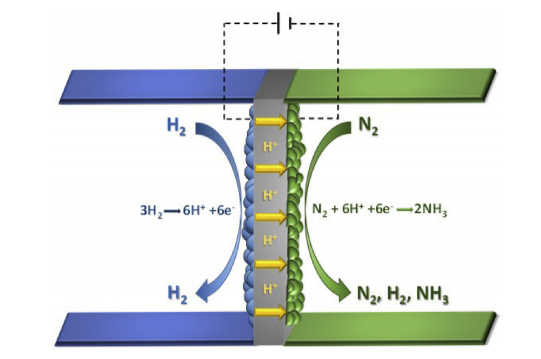
\includegraphics[scale=0.65]{electrochemical_synthesis}
			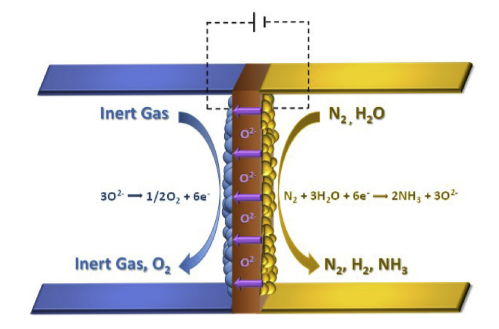
\includegraphics[scale=0.7]{electrochemical_synthesis2}	
			\caption{Electrochemical ammonia synthesis - anode (l), cathode (r)  \cite{Kyriakou2017}}
	}
%source https://ac.els-cdn.com/S0920586116304138/1-s2.0-S0920586116304138-main.pdf?_tid=04f1f2e8-973d-448d-aadd-175ff2e8e895&acdnat=1523822193_0cdd35a3744e5241062382a77c9c5f63%
\end{figure}}



\subsubsection{Photocatalytic Synthesis}
Using the same principles of photosynthesis the photocatalytic reaction of nitrogen and water to form ammonia and oxygen can be achieved at room temperature and atmospheric pressure with the addition of solar energy. However, despite ongoing research into this field and a number of photocatalysts available, the scale of this process would currently be unable to meet the ammonia requirement of the plant \cite{Liu2014}.

\subsubsection{Method Comparison}
Due to the diversity of methods available comparison of these methods will be done using multi-criteria analysis (Table \ref{tab:MCAJR}), due to the lack of comprehensive data from the electrocatalysis and photocatalysis methods. For simplicity the methods are given a design rating from 1-4 for each of the design objectives. These are then weighted to produce an overall rating for each of the reviewed methods. Safety was not included in this analysis due to the lack of comparative data.
\begin{table}[!htbp]
	\begin{center}
		
		\caption{Multi-criteria analysis table for reviewed ammonia synthesis methods \label{tab:MCAJR}}
		
		\begin{tabular}{|c|c|c|c|c|c|}
			\hline
			Method& Scale & Environmental & Economic   & Feasibility & Total \\ \hline
			Fe based Haber           & 4              & 3                          & 4 & 4             & \textbf{30}                     \\ \hline
			Ru based KAAP            & 4                & 3                        & 3 & 4         & 29                     \\ \hline
			Electrocatalysis            & 2                & 4                        & 2 & 2         & 20                     \\ \hline
			Photocatalytic synthesis            & 1                & 4                        & 1 & 1         & 14                  \\ \hline \hline
				\textbf{Weighting}& \textbf{2} & \textbf{2} & \textbf{1}   & \textbf{3} &  \\ \hline

		\end{tabular}
	\smallskip
	
	\textit{The Fe-based Haber process was chosen for the synthesis stage.}
	\end{center}
\end{table}

The weightings were justified with feasibility being the most important due to the need to ensure that only methods able to meet the technological requirements are used. Whilst new and emerging technologies were considered in the design process priority was given to methods that have been successfully implemented on medium and large scale processes, laboratory condition processes whilst considered were only chosen if there was a clear method in up-scaling to industrial levels and the benefits of doing so were significantly greater than established industrial processes. This was due to the need for reliability of power supply, especially considering the island location of the power plant and the lack of alternative power sources. The next most important considerations were environmental and scale requirements. This is due to the need to ensure that the methods are able to be scaled sufficiently without the need for large numbers of parallel systems. Environmental was also given a medium weighting of 2 due to its importance in the overall design requirements. Finally, economic was given the lowest ranking on this design process due to the fact that only comparative cost estimates can be found without specific design analysis. The sensitivity of the measurements to changes in score or weighting should also be considered. From the total results only the KAAP process is within 4 points of the Haber total, thus an single unit change in any one rating will only affect the overall optimum if the change was a direct improvement of the KAAP process over the Haber.

\subsection{Thermodynamic Modelling}
In order to make design choices a model for the synthesis of ammonia Haber process must be developed. To produce ammonia an exothermic reversible reaction takes place between hydrogen and nitrogen;
\begin{equation}
3H_2+N_2   \underset{ }{\stackrel{ }{\rightleftharpoons}}   2NH_3 \qquad \Delta h_0 = -92.44 \; kJ/mol 
\end{equation}

To better understand the nature of the reaction the thermodynamic are be considered in the following sections.


\subsubsection{Equilibrium Constant}

The equilibrium constant $K_a$ for ammonia synthesis was first calculated by Gillespie and Beattie (1930)\cite{Gillespie1930} and is a function of the reaction temperature $T$.
\begin{equation}
logK_a = -2.69log(T) - 5.52\times10^{-5}T + 1.85\times10^{-7}T^2+\frac{2001.6}{T}+2.69
%logK_a = -2.691122log(T) - 5.519265\times10^{-5}T + %1.848863\times10^{-7}T^2+\frac{2001.6}{T}+2.6899
\end{equation}
{\begin{figure}[h]
\begin{center}
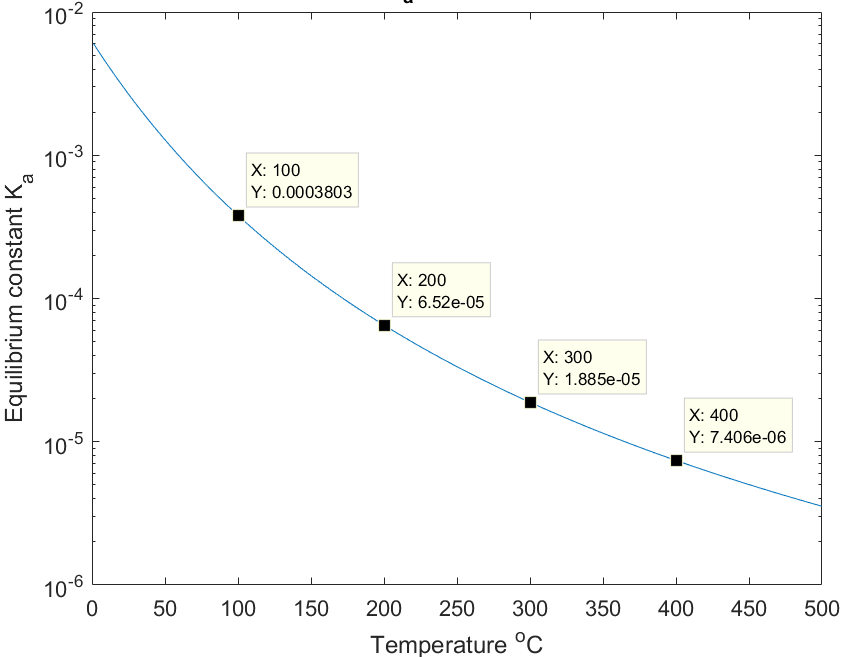
\includegraphics[scale=0.44]{K_a_varying_temperatureNEW}
		\caption{Equilibrium constant $K_a$ of ammonia synthesis reaction at varying temperature}
\end{center}
\end{figure}}

This clearly shows a decrease in the concentrations of products as the temperature increases; thus concurring with the Le Chatelier's principle that the equilibrium of reaction will shift to counteract the rise in temperature. This would suggest that a low reaction temperature would favour a high product yield at equilibrium. The governing mass balance within the reactor is:
\begin{equation}
 \dot{n}_{i,in}+\dot{n}_{i,form}=\dot{n}_{i,out}+\dot{n}_{i,accum}   
\end{equation}
where $\dot{n}_i$ are the molar flow rates for specie $i$, $\dot{n}_{i,in} = \dot{n}_{i,feed} + \dot{n}_{i,recycle} $ and $\dot{n}_{i,out} = \dot{n}_{i,prod} + \dot{n}_{i,recycle} + \dot{n}_{i,purge}$

\subsubsection{Reaction Mixtures}
When calculating the properties of N$_2$:H$_2$:NH$_3$ streams throughout the system a rule of mixtures is used. Eqn. \ref{eq:cpmix} gives the specific heat of a reaction mixture where $x_{i}$ are the mole fractions in the stream and $C_{p,i}$ are their respective specific heats. 
\begin{equation}
\label{eq:cpmix}
	C_{p,mix} = x_{N_2}C_{p,N_2} + x_{H_2}C_{p,H_2} + x_{NH_3}C_{p,NH_3}
\end{equation}
The specific heats  $C_{p,i}$ can be given by the polynomial temperature correlation, Eqn. \ref{eq:cp}.
\begin{equation}
\label{eq:cp}
C_{p,i} = a + bT + cT^2 + dT^3
\end{equation}

Clearly a Thermodynamic model alone would suggest that to produce high outputs of ammonia the reaction low temperatures should be chosen. However, this model is insufficient without also considering the rate at which this reaction would occur. 
\begin{table}[!htbp]
	\caption{Specific heat coefficients \cite{Morgan2013} \label{tab:cpco}}
	
	\begin{center}
		\begin{tabular}{|l|l|l|l|}
			\hline
			Coef. & 
			N$_2$               & H$_2$               & NH$_3$              \\
			\hline
			$a$           & $28.9$               & $29.11$              & $27.568$             \\
			\hline
			$b$           & $-0.1571*10^{-2}$ & $-0.1916*10^{-2}$ & $2.5630*10^{-2}$  \\ \hline
			$c$           & $0.8081*10^{-5}$  & $10.4003*10^{-5}$  & $0.99072*10^{-5}$ \\
			\hline
			$d$           & $-2.873*10^{-9}$  & $-0.8704*10^{-9}$ & $-6.6909*10^{-9}$ \\
			\hline
		\end{tabular}
		
	\end{center}
\end{table}

\subsection{Mechanism and Kinetics}

\begin{wrapfigure}{r}{0.25\textwidth}
	{\centering	
		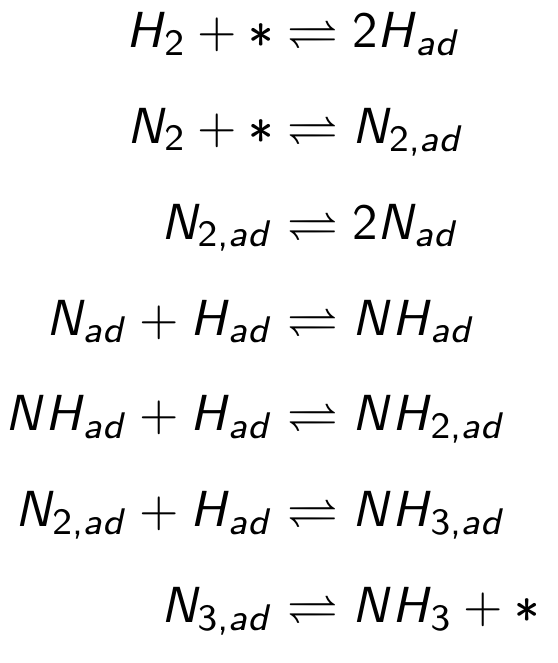
\includegraphics[width=1\textwidth]{mech}
		\caption{Synthesis mechanism \label{fig:mech}}
	}
\end{wrapfigure}
For a large scale process such as the Haber process with a large product output the rate at which the reaction occurs is a significant limitation on the product output of the plant. This is due to the fact that over a limited reaction time the reactants do not have sufficient time to reach a thermodynamic equilibrium.

\subsubsection{Reaction Mechanism}

The reaction mechanism of the ammonia synthesis stage was key in understanding the kinetics of reaction, determining the rate of reaction and the effectiveness of a catalyst. The mechanism for the synthesis reaction is shown in Fig. \ref{fig:mech} \cite{Jennings1991}.
%\begin{subequations}
%	{\singlespacing 	
%	\label{mech}
%\begin{align}
%H_2+*   &\underset{ }{\stackrel{ }{\rightleftharpoons}}   2H_{ad}\\
%N_2+*   &\underset{ }{\stackrel{ }{\rightleftharpoons}}   N_{2,ad}\\
%N_{2,ad}   &\underset{ }{\stackrel{ }{\rightleftharpoons}}   2N_{ad}\\
%N_{ad}+H_{ad}   &\underset{ }{\stackrel{ }{\rightleftharpoons}}   NH_{ad}\\
%NH_{ad}+H_{ad}   &\underset{ }{\stackrel{ }{\rightleftharpoons}}   NH_{2,ad}\\
%N_{2,ad}+H_{ad}   &\underset{ }{\stackrel{ }{\rightleftharpoons}}   NH_{3,ad}\\
%N_{3,ad}   &\underset{ }{\stackrel{ }{\rightleftharpoons}}   NH_{3}+*
%\end{align}
%}
%\end{subequations}

Where $*$ denotes the formation of an adsorption site. Experimental studies have found the adsorption of nitrogen to be rate determining in this process leading to an understanding of the microkinetics of the rate of reaction. This is due to the energy required to break the strong N$_2$ triple bond.

%As the reaction is exothermic an increase in temperature would favour the reactants over the products. Experimental studies have confirmed this. The equilibrium constant $K_a$ can be found using the Gillespie and Beattie equation;
%


\subsubsection{Rate of Reaction}

Numerous models \cite{Aparicio2008} for the synthesis rate of reaction $r$ have been established, however, the most widely used is the Temkin equation \cite{Guacci1977}. Since its discovery a number of different forms of the equation have now been developed. This analysis uses the Dyson and Simon form for its simplicity and the limited experimental data required to simulate results \cite{Dyson1968}.

\begin{equation}
\label{eq:GuiB}
r_{NH_3} = K_2 \left [ K_a^2 \times f_{N_2}
\left ( \frac{f_{H_2}^3}{f_{NH_3}^2} \right ) ^\alpha - \left ( \frac{f_{NH_3}^2}{f_{H_2}^3} \right ) ^{\alpha - 1}
\right ]
\end{equation}

Where the rate is a function of the fugacities $f$ , the well-known equilibrium constant $K_a$, empirical constant $\alpha$  and  $K_2$ defined by the Arrhenius law: where $k_20$ and $E_2$ are found experimentally and $R$ is the gas constant.
\begin{equation}
\label{eq:Arr}
	K_2 = k_{20}e^{-E_2/RT}
\end{equation}

{\begin{figure}[h]
		\centering
		{\centering	
		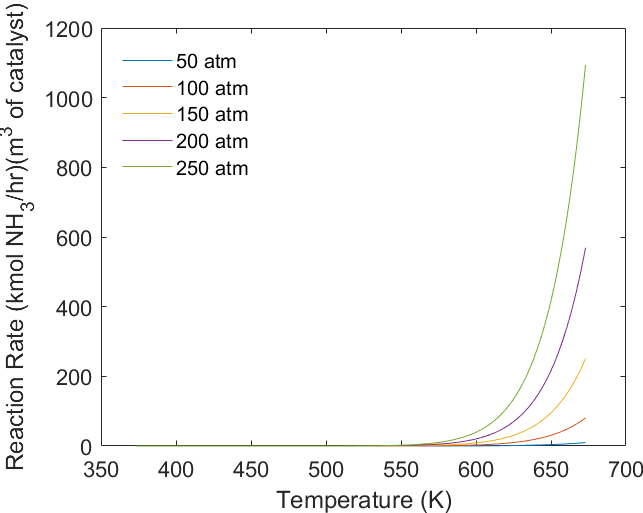
\includegraphics[scale=0.455]{reactionrate1}
		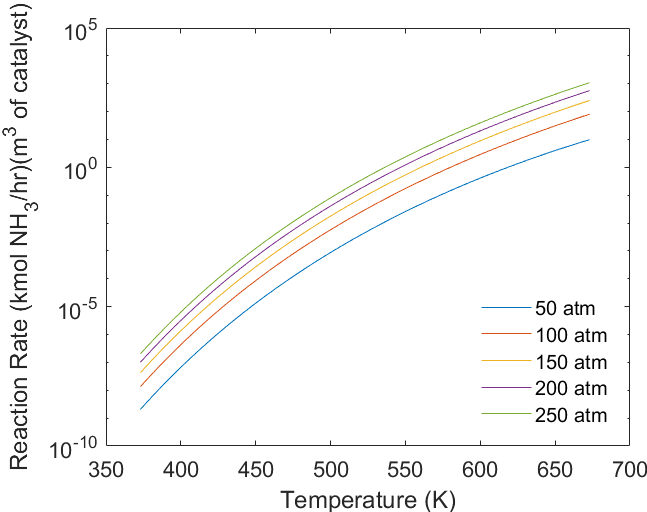
\includegraphics[scale=0.455]{LOGreactionrate1}	
		\caption{Reaction rate of ammonia synthesis \label{fig:rateGraph}}
		}

\end{figure}}


Figure \ref{fig:rateGraph} shows a significant increase in the rate of reaction as temperature increases, thus whilst the thermodynamic equilibrium decreases with temperature the rate of reaction increases. It is clear that as pressure increases the rate does also. The Temkin equation it is undefined when no ammonia is present due to the $f_{NH_3}$ term in the denominator. Clearly this does not follow the thermodynamic principles of a reverse reaction. Thus to resolve this a small amount ($\leq$1\%) of ammonia was included in the initial reactants; the reactor will be run at steady state conditions.

\subsubsection{Fugacities}
The fugacities $f_i$ of the respective gases can be calculated from the pressure $P$ and mole fraction of ammonia $Z$ using:

{\singlespacing
\begin{equation}
f_N{_2}= P\gamma_{N_2}\frac{a}{3\delta}(1-b_2Z)
\end{equation}
\begin{equation}
f_H{_2}=P\gamma_{H_2}a(1-b_1Z) 
\end{equation}
\begin{equation}
f_{NH{_3}}=P\gamma_{NH_3}\times Z 
\end{equation}}


Where $a= \frac{3\delta}{3+ 1}$,   $ b_1 = \frac{i_0 +0.5 + (0.5/\delta)}{1-i_0}$, $ b_2 = \frac{i_0 - 0.5 +1.5\delta}{1-i_0}$ and $3\delta$ is the H/N ratio.
Fugacity coeffiecients $\gamma$ can be calculated using the Cooper (1967) and Newton (1935) expressions given as:

	{\singlespacing 
\begin{equation} \gamma_{N_2} = 0.93432 + 0.3102\times10^{-3}T+0.2959\times10^{-3}P-0.2707\times10^{-6}T^2+0.4775\times10^{-6}  P^2
\end{equation}
\begin{equation} 
\gamma_{H_2} = exp\{ e^{-3.840T^{0.125}+0.541}P-e^{-0.126T^{0.5}-15.98}P^2+300[e^{-0.01190T-5.94}](e^{-P/300}-1)\}
\end{equation}
\begin{equation} 
\gamma_{NH_3} =0.1439 + 0.2029\times10^{-2}T - 0.4488\times10^{-3}P - 0.1143\times10^{-5}T^2 + 0.2761\times10^{-6}P^2
\end{equation} }
\begin{wrapfigure}{r}{0.6\textwidth}
		\centering
		
		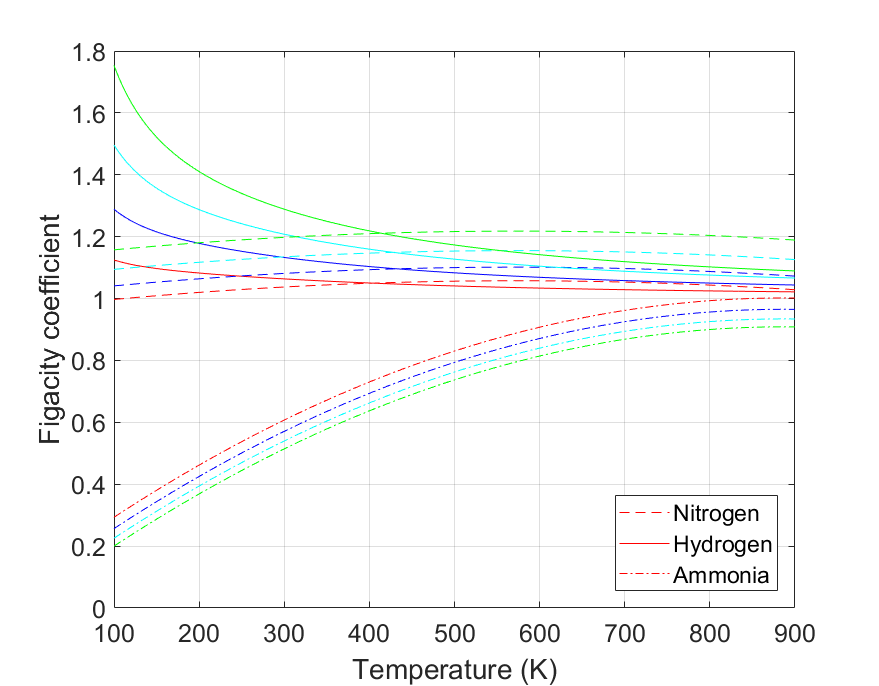
\includegraphics[width=1\textwidth]{fugacity_coeff1}
		\caption{Variation of fugacity coefficients with temperature \label{fig:fugco}}
\end{wrapfigure}
The sensitivity of the fugacity coefficients to temperature can be seen on Figure \ref{fig:fugco}. This shows that as temperature decreases and pressure increases the behaviour of gases becomes increasingly non-ideal. 


\subsubsection{Modelling}
The kinetics were implemented in ASPEN using a Langmuir-Hinshelwood-Hougen-Watson (LHHW) model, simulating the surface mechanisms during reaction. This is commonly used for modelling heterogeneous reactions with a solid catalyst and fluid reactants. For ASPEN simulation the model must be given in the form \cite{Plus2008}:
\begin{equation} 
\text{Rate} = \frac{\text{(Kinetic factor)(Driving force)}}{\text{(Absorption)}}
\end{equation}


In this form and using the Dyson and Simon form of the Temkin equation the absorption term can be set to unity and the kinetic factor to $K_{2}$, giving a driving force expression: 
\begin{equation} \text{Driving force} = K_a^2 \times f_{N_2}
f_{H_2}^{3\alpha}f_{NH_3}^{-2\alpha} - f_{NH_3}^{(2\alpha-2)}f_{H_2}^{(3-3\alpha)} \end{equation}

Using the experimental values for $k_{20}$ and $E_2$ in Eq. \ref{eq:Arr} to calculate $K_2$ and then the Gillespie and Beattie equation (Eq. \ref{eq:GuiB}) to calculate $K_a$ and an experimental value of $\alpha = 0.5$ a kinetic model for the reaction was formed. Initial simulations of this model in a PFR reactor in aspen at a first approximation of industrial conditions (p=100bar T=400\textdegree C) giving a first pass conversion of $\approx25\% $ NH$_3$.

\subsection{Catalyst}

In modelling the rate of reaction Dyson and Simon accounted for the flow of reactants through a reactor. To account for the presence of a solid catalyst an effectiveness factor $\xi_{c}$ was used such that an effective rate ($r_{eff}=\xi_{c}r_{NH_3}$) through the reactor could be calculated using the following assumptions \cite{Dyson1968}; The catalyst particles can be considered as spheres. The diffusion coefficients of each component are independent of position within a particle, particles are isothermal and Knudsen diffusion is not experienced. Giving the equation:
\begin{equation}
	\xi_{c} = \frac{(\text{molar flux of component i across surface})\times(\text{surface area of catalyst pellet})}{(\text{vol. of catalyst pellet})\times(\text{rate of formation of component i at surface})}
\end{equation}

\begin{wraptable}{r}{0.4\textwidth}
	{\singlespacing
\centering
		\caption{W\"{u}stite catalyst \cite{Pernicone2003}}
		\begin{tabular}{ |l|l|  }
			\hline
			A301 particle size & 1.5-3.0mm\\
			\hline
			Bulk density & 3.25 g/cm$^3$\\
			\hline
			BET surface area & 16.6 m$^2$/g\\
			\hline
			K$_{20}$&  0.874 x 10$^{16}$\\
			\hline
			E$_2$ &44.9 kcal/mol \\
			\hline
		\end{tabular}
}
\end{wraptable}
Throughout the past 100 years an Fe-based magnetite (Fe$_{2}$O$_3$) precursor with a variety of oxidic promoters have been the principal catalyst used industrially in ammonia synthesis \cite{Liu2014}. However, recently a number of additional catalysts have been developed; involving the use of a various other materials as promoters including ruthenium and bimetallic nitrides. These were considered during the initial design of the plant due to their higher yields of ammonia at reduced pressures, but drawbacks included both the high cost and limited availability in the case of ruthenium. Considering the island location of the power generation facility the availability of resources was a key factor in the choice of catalyst. On balance, the additional cost of these materials are substantially higher than iron and thus greatly increase both the initial capital costs of the plant but also the running costs of the plant due to the increased material costs. Thus an alternative w\"{u}stite (Fe$_{1-x}$O) iron catalyst was chosen for the ammonia synthesis stage. This was chosen due to the increased reaction rate at lower operating pressure than the traditional magnetite promoter thus reducing the pressure needed for the reactor and the capital costs required. The catalyst in use will be the A301 catalyst manufactured by Shangyou Catalyst Co. Ltd. 

\begin{table}[!htbp]
	\begin{center}
		\caption{A301 Catalyst composition}
		\begin{tabular}{ |c|c|c|c|c|c| }
			
			\hline
			\textbf{Compound} &Fe oxide & Al$_2$O$_3$ & K$_2$O & CaO & Others*\\
				\hline
			\textbf{A301 (\%)} &93.0 & 2.7 & 0.8 & 2.8 & 0.7\\
			\hline
		\end{tabular}
	\small
	\\
	*Impurities in raw material
	\end{center}
\end{table}

\subsection{Reactor Design}
\begin{wrapfigure}{r}{0.41\textwidth}
		\centering
		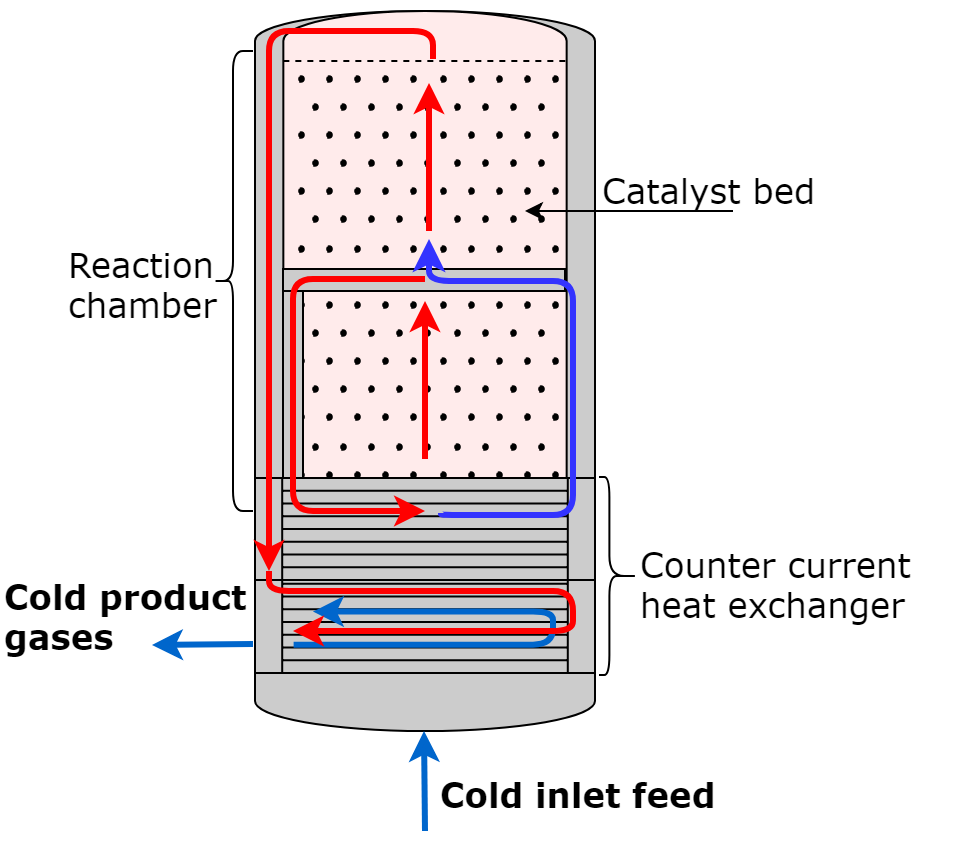
\includegraphics[width=\textwidth]{2sReactorP.png}
		\caption{Two stage reactor}
\end{wrapfigure}

The synthesis reactor is central to the design of the process as it is within that the synthesis reaction takes place. In order to maintain close to optimum conditions  a two bed reactor with intercooling between them was chosen. This enables the products of the first bed to return to a lower temperature before entering the second stage.

\subsubsection{Reactor Sizing}
The reactor consists of two reactor stages with interstage indirect cooling. Both reactor inlet stages are designed as fixed bed reactors with an even catalyst spacing throughout. 

The overall volume of the reactor V, can be given by Eq. \ref{eq:reacsize}: where $r$ is the rate of reaction, $\rho_{cat}$ is the packing density of the catalyst and $\dot{m}$ the mass flow rate \cite{Banares-alcantara2014}.
\begin{equation}
\label{eq:reacsize}
	V = \frac{\dot{m}}{1000\rho_{cat}r}
\end{equation}
Rearranging the steady flow energy equation for an adiabatic reactor with no shaft work ($Q,W_s=0$) gives an energy balance within the reactor: where $\Delta H_{reac}$ is the heat of reaction per mol$_{NH_3}$ and x is the distance along the reactor.
\begin{equation}
\frac{\dd T_{reac}}{\dd x} = \frac{(-\Delta H_{reac})A_{cat}}{\dot{m}_{mix}C_{p_mix}}r_{NH_3}
\end{equation}

\begin{table}[!htbp]
	\begin{center}
		\caption{Reactor sizing\label{tab:reacreq}}
		\begin{tabular}{|c|c|c|c|c|c|}
			\hline
			Reaction rate r& $\rho_{cat}$ & $\dot{m}_{NH_3}$ & V  & L$_T$ & D$_T$ \\ \hline
			$1.3838*10^{-4}$ $\frac{kg_{NH_3}}{s^{-1}kg_{cat}^{-1}}$       & 3.25 kg/L         & 3.22 kg/s                      & 7.16 m$^3$ & 2.74 m & 1.83 m \\ \hline
		\end{tabular}
	\end{center}
\end{table}

\subsubsection{Dimensions and Pressure Drop}

Pressure drop across a reactor can be calculated using the Ergun equation \cite{Ergun1949}:

\begin{equation}
\frac{\Delta p}{L}= \frac{150\mu(1-\epsilon)^2}{D_p^2\epsilon ^3}v_s+\frac{1.75(1-\epsilon)\rho}{D_p\epsilon ^3}v_s^2
\end{equation}
where $\Delta p$ is the pressure drop across the length $L$ of the bed, $\mu$ is the fluid viscosity, $\epsilon$ is the void space in the bed (taken as $\epsilon = 0.5$ \cite{Ergun1949}), $\rho$ is the density of the fluid, $D_p$ is the particle diameter and $v_s$ is the superficial velocity of the fluid where $v_s = \frac{Q}{A} = \frac{\text{volumetric flow rate}}{\text{bed cross sectional area}}$.
\begin{table}[!htbp]
	\begin{center}
		\caption{Reactor dimensions and pressure drop}
		\begin{tabular}{ |p{2.3cm}|p{2.3cm}|p{2.3cm}|p{2.3cm}|p{2.7cm}|p{2.3cm}| }
			\hline
			
			Reactor bed & Volume m$^3$& Length m&Diameter m&Thickness mm&$\Delta p$ atm\\
			\hline
			1&3.28 & 1.25 &1.83 &47.0& 4.30\\
			\hline
			2&3.91 & 1.49 &1.83 &47.0&4.08\\
			
			\hline
		\end{tabular}
	\end{center}
\end{table}


Modelling the outlet temperature against reactor length in Figure \ref{fig:Rlen} for a single bed with an input temperature of 400 \textdegree C and a diameter D$_1$ = 1.83 m shows a change in the reactor profile up to L$_1$=1.25 m: after this point increasing the reactor length no longer increases the NH$_3$ yield thus this was chosen as a suitable length for the first stage. Using this first stage design a second bed could be subsequently designed; a larger bed was required to optimise ammonia yield. Simulating the reactor bed on ASPEN an optimum length of D$_2$=1.82 m and L$_2$=1.49 m was chosen as after this point there was no significant increase in performance with reactor length, giving a first pass conversion of 34.2\% \cite{Elnashaie1989}. Furthermore, under a reactor pressure of $\pbar$  bar the thickness of the walls must be sufficient to withstand the high internal pressures of reaction.

{\begin{figure}[!htbp]
		
		\centering
		
		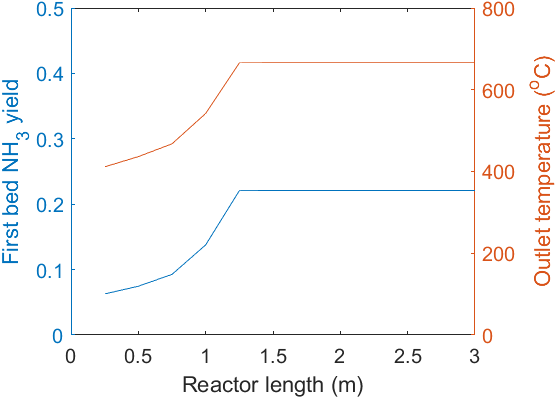
\includegraphics[width=0.49\textwidth]{length1}
		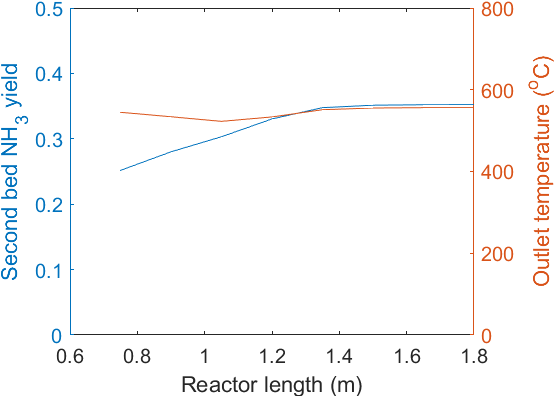
\includegraphics[width=0.49\textwidth]{length2}
		\caption{First (l) and second (r) reactor temperature and yield profile with length \label{fig:Rlen}}
	\end{figure}
}

\subsubsection{Material Selection}
In order to calculate the thickness of material required  the internal reactor forces must be measured, as must the operating temperatures. Simulation shows the peak temperature of normal operation of the reactor remains below 700\textdegree C. Therefore a material with a melting point significantly higher than this is required. Due to the corrosivity of NH$_3$ to a number of metals high-yield steel was chosen as the material for construction of the vessel. 
\begin{table}[!htbp]
	\begin{center}
		\label{tab:matreq}
		\caption{Properties of high yield steel \cite{Howatson1972}}
		
		\begin{tabular}{|c|c|c|c|c|}
			\hline
			Density& Melting point & Yield stress & Ultimate tensile strength& Cost    \\ \hline
			7850 kg/m$^3$       & 1500\textdegree C          & 400 MPa                          & 600 MPa&\$896/ton \cite{Meps2018} \\ \hline
		\end{tabular}
		
	\end{center}
\end{table}

To ensure the reactor material can withstand the reactor pressures it must both withstand the hoop and longitudinal stresses within the reactor such that:
\begin{equation}
\frac{\sigma_{yield}}{S.F.} \geq \sigma_L=\frac{PD}{4t} \text{  and  } \frac{\sigma_{yield}}{S.F.} \geq \sigma_H=\frac{PD}{2t}
\end{equation}
where a safety factor of 2 is taken. This gives the condition that for high yield steel t $\geq 46.9\ mm$, the thickness of the vessel is taken to be $47\ mm$. For the leak before break failure condition: where $B$ is wall thickness and $K_c$ is the critical stress intensity factor.
\begin{equation}
\sigma_{yield}<\frac{K_c}{(\pi B)^{0.5}}
\end{equation}



\subsubsection{Heat Exchanger}

For the two stage reactor design intermediary cooling is key factor in ensuring the exothermic synthesis reaction does not result in an unwanted temperature increase, thus shifting the equilibrium of reaction further towards the reactants. There were two main methods considered in literature. These were direct quench cooling and heat exchanger indirect cooling.

\subsubsubsection{Quench Cooling}
Direct quench cooling involves the addition of cold feed mixtures during the reactor stages in order to reduce the reactor temperature at each stage. This means that only a fraction of the total feed enters the first reactor stage.
\subsubsubsection{Indirect Cooling}
Indirect cooling involves a heat exchanger passing the hot product gases past the cold feed gases in order to raise the temperature of the feed gases. This means the entire feed stream passes through all reactor stages and thus the time in the reactor is maximised.
\subsubsubsection{Design}
The chosen method for cooling configuration was the indirect cooling due to the maximisation of reaction time. This is supported by empirical analysis \cite{Penkuhn2017}. The heat exchanger used in the reactor is a counter-current heat exchanger with steady state heat transfer. From this it is possible to derive an energy balance equation \cite{Jinasena2016};
\begin{equation}
\frac{dT_c}{dx}=\frac{UA}{\dot m_i C^i_pL}(T_h-T_c)  
\end{equation}
\begin{equation}
\frac{dT_h}{dx}=\frac{UA}{\dot m_o C^o_pL}(T_h-T_c)
\end{equation}
In which $T_c$ and $T_h$ are the respective cold inlet and hot outlet streams. $A$ is the area for heat transfer to occur and $U$ is the overall heat transfer coefficient of the heat exchanger (290.35Wm$^{-2}K^{-1}$)\cite{Elnashaie1988}, whilst $C_p$ are the specific heat capacities for the respective inlet and outlet streams of gas mixtures (Eqn. \ref{eq:cpmix}) and $\dot m$ are the mass flow rates of the respective streams. Along a heat exchanger of length $L$ where $x$ is the relative position along it. If we then assume $\dot m_i c^i_p$ is equal to $\dot m_o c^o_p$ and similarly $\frac{UA}{\dot m_i c^i_p}$ does not depend on $x$; then the above expressions can be simplified in order to give the temperature at the reactor inlet and outlet:
\begin{equation}
T_r^i = \frac{T_i + \frac{UA}{\dot m_i C^i_p}T_r^o}{1+\frac{UA}{\dot m_i C^i_p}}
\end{equation}
\begin{equation}
T_o = \frac{T_r^o + \frac{UA}{\dot m_i C^i_p}T_i}{1+\frac{UA}{\dot m_i C^i_p}}
\end{equation}

The aim of the heat exchanger is twofold. The first of these is to heat up the feed of the product gases to a significantly high temperature to allow for a suitable rate of reaction. This is done by running the hot product gases in counter current to the feed gases. The second use of the heat exchanger is in a two-stage reactor system as an intermediary cooler for the product gases. This brings the temperature down to one in which the reaction equilibrium maintains a increased fraction of ammonia products.

\subsection{Additional Units}

\subsubsection{Separator}

In order to remove the fraction of ammonia from the product mixture, the relatively high boiling point of ammonia was used to remove liquid ammonia at high pressure and low temperature in a separator. This separates liquid droplets from gas particles by using gravity separation to allow the gaseous products to leave from the top outlet whilst liquid ammonia is removed from the bottom outlet in a vertical separator ( Fig. \ref{fig:sep}).

\begin{wrapfigure}{r}{0.33\textwidth}
	\centering
	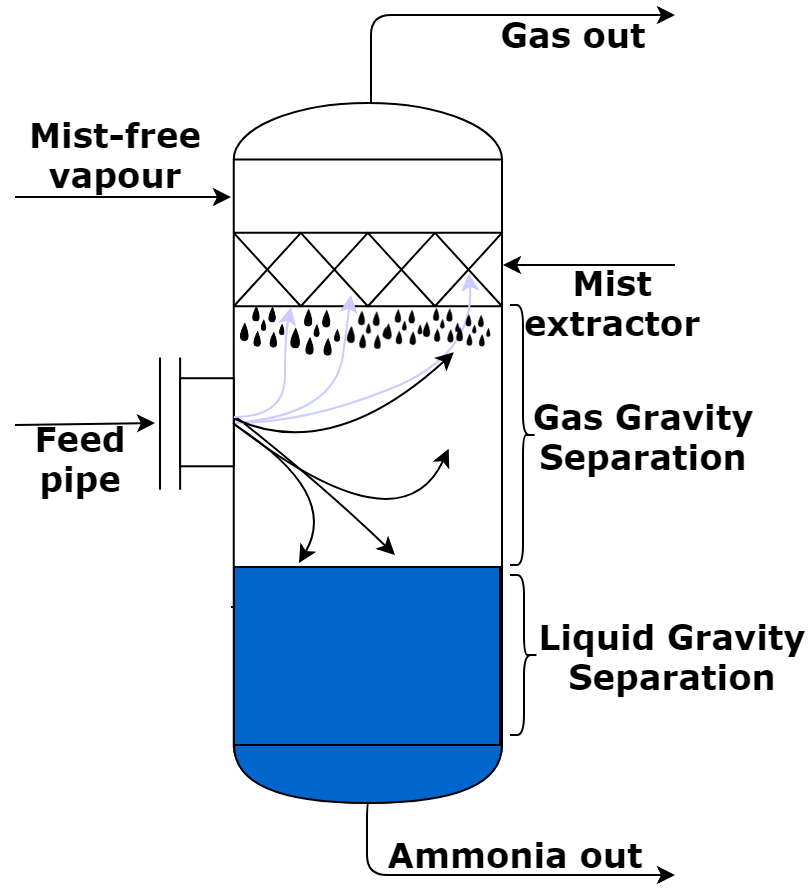
\includegraphics[width=0.99\textwidth]{CondenserPRESENTATION}
	\caption{Vertical separator \label{fig:sep}}
\end{wrapfigure}

To separate liquid ammonia from the product gases The Souders-Brown design equations were used to equate the drag force $F_D$ exerted by gas flow to the gravity force of the droplet weight $F_G$ \cite{Campbell2015} \cite{Jekel2001}. Assuming plug flow $F_D = F_G$. Substitution of expressions for the forces on a spherical droplet give the maximum gas velocity, V${_G}_{max}$ using the Souders-Brown method \cite{Souders1934}; K$_s$ is found experimentally.

\begin{equation} V_{Gmax}=K_s\sqrt{ \left ( \frac{\rho_L - \rho_G}{\rho_G} \right )}\  when \  K_s = \sqrt{ \left ( \frac{4gD_P}{3C_D} \right )} \end{equation}

\begin{equation}D_{min} = \sqrt{\left ( \frac{(4/\pi)q_a}{F_GV_Gmax} \right ) } \end{equation}
\\ 
Using a mist extractor - a horizontal wire mesh pad in a vertical separator used to coalesce the liquid into droplets large enough to drop from the mesh pad, $K_s = 0.12$. For a length/diameter ratio of 4/1 to reduce the material required in construction. And using a industrial standard HY-80 steel the separator can be modelled as a thin walled pressure vessel to calculate the required wall thickness of the tank \cite{Howatson1972}.
\begin{equation}
	\sigma_{yield}=\frac{pr}{t}
\end{equation}
For an internal pressure of 140 bar, known material and dimensions of the separator can be sized.

\begin{table}[!htbp]
	\begin{center}
		\caption{Separator design summary}
		\begin{tabular}{ |c|c|c|c|c|c| }
			\hline
			
			$K_s$ & V${_G}_{max}$&D$_{min}$ &F$_G$& H & Vol \\
			\hline
			0.12& 74kW & 0.594 m &1 & 2.296 m & 0.636 m$^3$\\
			
			
			\hline
		\end{tabular}
	\end{center}
\end{table}
\subsubsection{Compressor}
In order to obtain the high operating pressures required for ammonia synthesis centrifugal compressors are used both in the feed streams and in the reactor inlet stream. The feed compressor is used to raise the pressure of the feed gases to the pressure of the recycle stream. Whilst the reactor inlet compressor raises the pressure to account for the pressure drop across the reactor. In this analysis the compressors are assumed to be driven by electric motors, however, turbine powered compressors are also possible, had the gas turbine generator been run continuously for power generation, this would also have been considered. 
For an isentropic compressor the total output temperature can be calculated from Eqn. \ref{eq:compT} \cite{Morgan2013}.
\begin{equation}
\label{eq:compT}
T_{out} = T_{in}\left[ \left( \frac{P_2}{P_1}\right)^{\frac{1}{N}} \right]^{\left( \frac{n-1}{n}\right)} 
\end{equation}
The total 
compression power required $\dot W_{comp}$ is given by Eqn. \ref{eq:compP}
\begin{equation}
\label{eq:compP}
\dot W_{comp} = \frac{ \dot W_{fluid}}{\eta_{comp}} = \frac{1}{\eta_{comp}} TN\frac{n}{n-1}R\dot m \left( \left[ \left( \frac{P_2}{P_1}\right)^{\frac{1}{N}} \right]^{\left( \frac{n-1}{n}\right)} - 1 \right)
\end{equation}
Where $T$ is the input temperature, $N$ is the number of compressor stages, $n$ is the polytropic exponent, $R$ the specific gas constant, $\dot m$ is the mass flow rate and $P_1$ and $P_2$ are the respective inlet and outlet pressures. $\eta_{comp}$ is the overall compressor efficiency which the product of mechanical and isentropic efficiencies such that $\eta_{comp} =\eta_{is}\eta_{m}$. Standard efficiences of centrifugal compressors are taken as $\eta_{is} = 0.85$ and $\eta_m = 0.95$ \cite{Penkuhn2017}. 

\begin{table}[!htbp]
	\begin{center}
		\label{tab:power}
		\caption{Combined compressor power requirements of plant}
		
		\begin{tabular}{|c|c|c|c|c|c|c|c|c|}
			\hline
			Compressor& $T_{in}$ (K)& $n$ & $P_2/P_1$ & N & $\dot{W}_{fluid}$ & $\dot{W}_{comp}$\\ \hline
			1      &298          & 1.40                & 25 &2 & 1084 kW & 1342 kW\\ \hline
			2& 513 &  1.40 & 5.6  & 2& 892 kW & 1104 kW\\ \hline
			3      & 565         & 1.40                 & 1.07 &1 &77 kW & 95 kW \\ \hline
				\textbf{Total}      &          &                  &  &  & \textbf{2053 kW}&\textbf{2541 kW}  \\ \hline
		\end{tabular}
		
	\end{center}
\end{table}

The total cooling power, $\dot{Q}$ can be found in order to size the intercooling heat exchangers: where $C_{p,mix}$ is found from Equation \ref{eq:cpmix}.


\begin{equation}
\label{eq:coolpowerQ}
\dot{Q} =\dot{m}(N-1)(T_{out}-T_{in})C_{p,mix}
\end{equation}

%
%\begin{table}[!htbp]
%	\begin{center}
%		\label{power}
%		\caption{Combined compressor power requirements of plant}
%		
%		\begin{tabular}{|c|c|c|c|}
%			\hline
%			Plant size (t/day)& Total fluid power & Shaft power & Driver power\\ \hline
%			250      &6.36MW         & 7.47MW                        & 7.86MW  \\ \hline
%		\end{tabular}
%		
%	\end{center}
%\end{table}
%
%


\subsubsection{Purge}
In order to limit the build-up of inert gases within the synthesis loop, a fraction of the recycle loop is purged. However, due to the cost of obtaining feed gases it is beneficial to keep the purge fraction small. After simulating a number of purge fractions on ASPEN a fraction of \purge \%  of the recycle stream was chosen. This purge stream is comprised of mostly H$_2$ and N$_2$ feed gases. Considering the high energy requirement of the electrolyser hydrogen recovery of this stream is in both environmental and economic interest. For this stage there are two main methods; membrane technology and cryogenic separation, with the former generally requiring a lower initial investment whilst the latter provides a greater energy efficiency \cite{Ojha2010}. Further economic evaluation of this process is outside the scope of this design.

\subsection{Ammonia Storage}
\label{subsec:JRstorage}

Storage of liquid ammonia product is vital in matching the supply and demand sides of the plant. Thus the scale of this storage must be one of the largest stores in the plant. Liquid ammonia has a boiling point of -33.3\textdegree C at atmospheric conditions, however, this can be increased by pressure storage. This requires a compromise to be made between low temperatures and high pressures in which to store ammonia. A review of current large-scale ammonia storage methods (Bartels,2008)\cite{Bartels2008} highlights the main trade-off between high pressure and low temperature storage being the high capital cost of building high pressure vessels against the increased energy requirements and thus running costs of maintaining low temperature storage.

\begin{wrapfigure}{r}{0.4\textwidth}
	\centering
	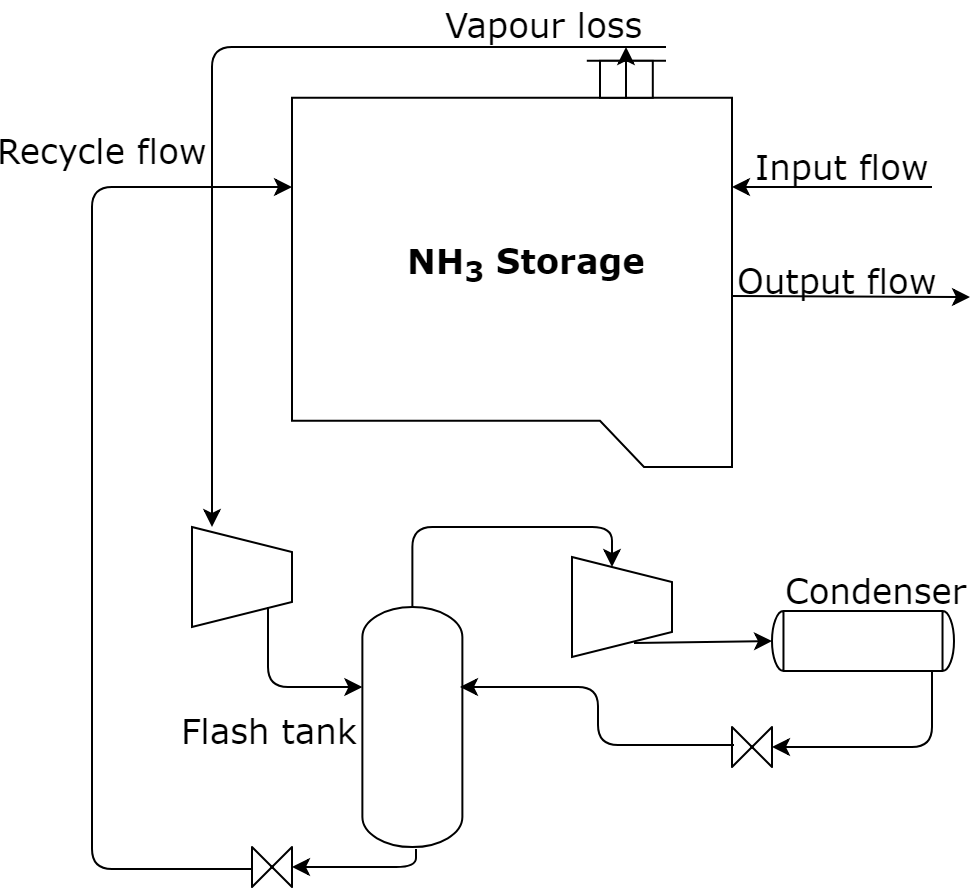
\includegraphics[width=0.99\textwidth]{AmmStoreP}
	\caption{Cold NH$_3$ storage cycle}
\end{wrapfigure}
As calculated in  section \ref{sec:plantscale} the maximum capacity for required ammonia storage is 15000 tonnes at maximum capacity.

\subsubsection{Low Temperature Storage}

Storage of NH$_3$ at low temperature and ambient pressure is commonly used for large scale storage due to higher ammonia/steel ratio and thus a reduction in capital cost. At atmospheric pressure approximately 43 tonnes of ammonia can be stored per tonne of steel. This massively reduces the capital cost on steel. Despite this other factors must also be considered, mainly boil-off rate due to heat transfer from the environment. The mass of evaporated ammonia and thus the boil-off rate is given as;
\begin{equation}
{\text{NH}_3}_{evap} = \frac{\dot{Q}}{\Delta H_{vap}}
\end{equation}
\begin{equation}
\text{Boil-off (\%)} = \frac{{NH_3}_{evap} }{{NH_3}_{storage} }
\end{equation}
This is typically below a conservative estimate of 0.1\% per day \cite{Belapurkar2016}. Giving a maximum boil-off of 15 t/d. Using an ammonia refrigeration cycle system for 15000 tonnes a storage tank of at least $21.997\times10^3$ m$^3$ would be required (density of liquid ammonia, $\rho_{NH_3(l)}$=681.9 $kg/m^3$)\cite{Hacker2003}. 

\subsubsection{High Pressure Storage}

Pressure storage does not suffer from evaporation losses or cooling costs. However, it is limited by its structural mechanics and this material used for construction of the pressure vessel. To increase capacity more vessels are required. Bartels shows that in order to store ammonia at an ambient temperature of 20$^o$C, a pressure of 8.58 bar would need to be maintained. However, the limiting size of a steel pressure vessel is calculated to be approximately 270t. The recommended ratio is about 2.8 ton NH$_3$ stored for every tonne of steel. 

\subsubsection{Design}
High pressure storage would require 55 pressure vessels using over 5000 tonnes of steel, thus cold storage is a preferred option due to environmental and economic benefits. 

\begin{table}[!htbp]
	\begin{center}
		\caption{Comparison of ammonia storage methods}
		\begin{tabular}{ |c||c||c|| }
			\hline
			\multicolumn{3}{|c|}{Ammonia Storage - 15000 tonnes required } \\
			\hline
			
			Properties & High pressure& Low temperature\\
			\hline
			NH$_3$ Energy density (MJ/L) & 13.77& 15.37\\
			Ammonia/Steel ratio & 2.8& 43\\
			Pressure required (bar) & 8.58 &Atmospheric\\
			Temperature required ($^o$C)& 20 &-33.3\\
			Storage efficiency&100\%&96.3\% \\
			
			Tanks required   &55&1 \\
			Steel required (tonnes)   &5357&349 \\
			
			
			\hline
		\end{tabular}
		\\
	
		
	\end{center}
	
\end{table}

%https://lib.dr.iastate.edu/cgi/viewcontent.cgi?referer=https://www.google.co.uk/&httpsredir=1&article=2119&context=etd%

In order to minimise the heat transfer the surface area/volume ratio of the storage tank must be minimised. Despite the optimal ratio of a spherical tank the 3d nature of the shape would cause significant structural issues in building a sufficiently large container, thus a 3D projection of a 2 dimensional shape is preferred for vertical support. The optimal shape of this design is a cylindrical storage tank. For a maximum volume of $21.997\times10^3$ m$^3$ the optimum radius/height ratio is $\frac{h}{r} = 2$ giving a radius, r $ = 15.184$m and height, h $ = 30.38$m steel containers. Insulated double containment tanks are used to minimise heat transfer and to ensure toxic vapours are not released in the case a rupture. The outer tank is made from concrete. Estimation of the hydrostatic pressure at the bottom of the storage container can be given by the equation:
\begin{equation}
P_h= \rho g h
\end{equation}
In the case of ammonia the pressure on the bottom of the tank would be 203.144 MPa of additional pressure. Thus a suitable steel thickness would have to be chosen to withstand this. Designing the refrigeration system using the compressor design equations and with a flash tank liquid holdup time of 10m the condenser can be sized using \cite{Morgan2013}; where H is the specific mass enthalpy.
\begin{equation}
	\text{Area} = \frac{\dot{m}H}{U_{cond}T_{LMTD}}
\end{equation}

\begin{table}[!htbp]
	\begin{center}
		\caption{Storage refrigeration cycle design summary}
		\begin{tabular}{ |c|c|c|c| }
			\hline
			
			Flow rate $\dot{m}$ & Compressor power&Flash volume &Condenser area\\
			\hline
			0.17 kg/s& 74kW & 0.31 m$^3$ &69.7 m$^2$ \\
		
			\hline
		\end{tabular}
	\end{center}
\end{table}
\subsection{Ammonia Cracker}
In order to produce feed gases for the gas turbine the liquid ammonia must first be decomposed into N$_2$ and H$_2$ in the endothermic reaction \cite{Kim2012}. 
\begin{equation}
2NH_3   \underset{ }{\stackrel{ }{\rightleftharpoons}}   3H_2 + N_2 \qquad \Delta h_0 = 46 kJ/mol 
\end{equation}

\begin{wrapfigure}{r}{0.36\textwidth}
	\centering
	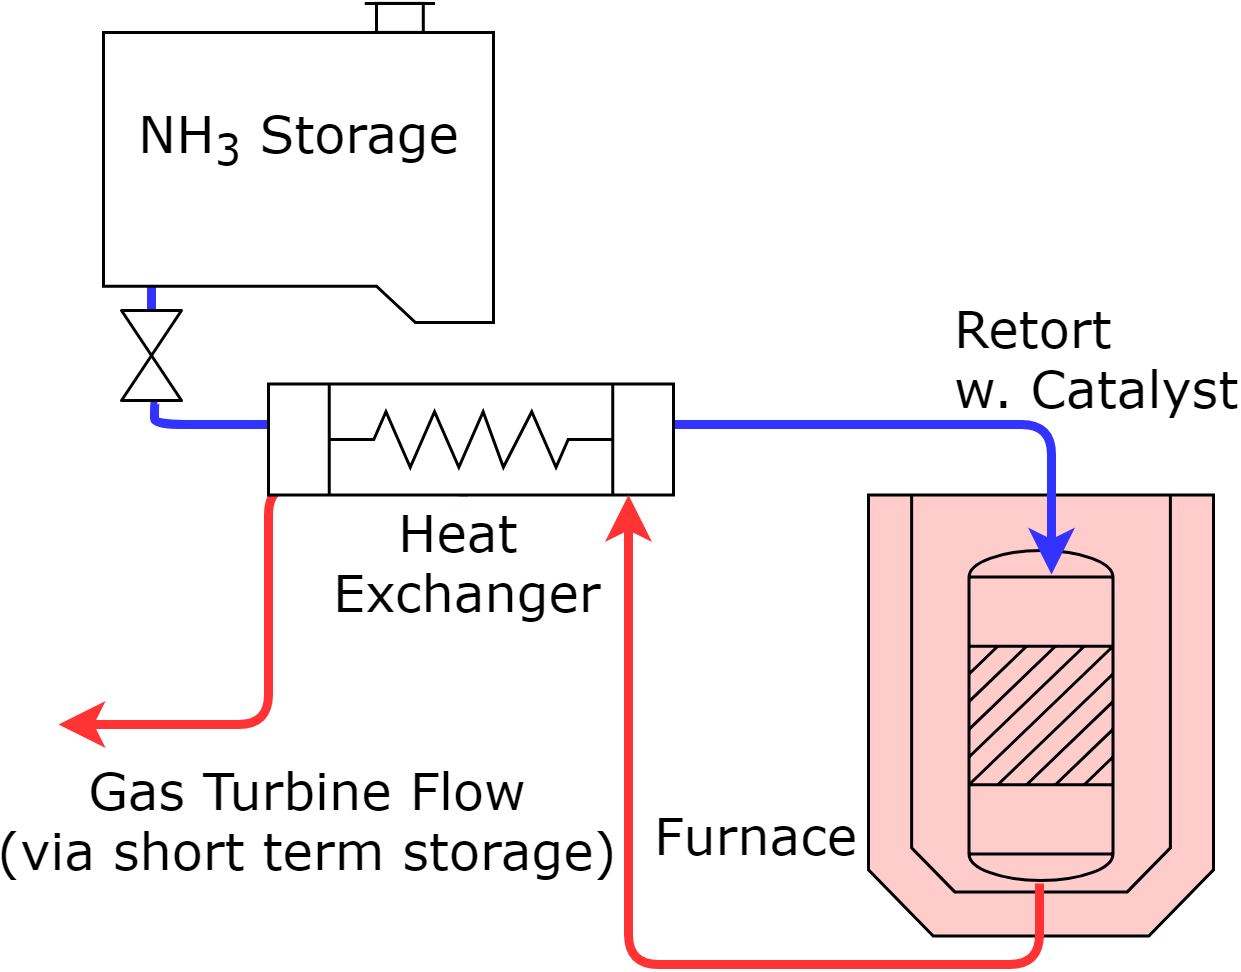
\includegraphics[width=0.99\textwidth]{ammcrack}
	\caption{Ammonia cracker flow network}
\end{wrapfigure}

This requires the addition of heat due to the endothermic nature of the reaction and thus must be conducted in a furnace with a nickel catalyst to achieve the conversions required for decomposition.

Due to the high peak demands of the 3 gas turbines a small amount of the cracked gas is stored. This is done to reduce the peak requirement of the cracker. The standard capacity of an industrial cracker is 1000 m$^3$/h at operating conditions the plant would require 26 SINCE-GAS ANH units  at a cost of \$260000 per unit \cite{SinceGas2018}. 

\begin{table}[!htbp]
	\begin{center}
		\caption{Ammonia cracker design requirements}
		\begin{tabular}{ |l|l|  }
			
			\hline
			Peak NH$_3$ mass flow demand & 32.815 kg/s\\
			\hline
			Average NH$_3$ mass flow rate required & 0.1648 kg/s\\
			\hline
			Ramp-up time of SOFC&  0.5h\\
			\hline
			Maximum theoretical capacity required& 59067 kg/SOFC ramp-up\\
			\hline
			Minimum turbine down-time    &2h \\
			\hline
			Capacity requirement of cracker& 5.469 kg/s\\
			\hline
			Cracked gas storage requirement & 49.223 ton \\
			\hline
			Total cost of cracker & \$6,760,000 \\
			\hline
			Operating pressure & 0.5 - 1.0 bar \\
			\hline
		\end{tabular}
	\end{center}
\end{table}


\subsection{Modelling, Optimising and Control}
This section addresses the methods used in modelling, optimising and controlling the process in order to achieve peak operating conditions.

{\begin{figure}[!htbp]
	%	{\centering
			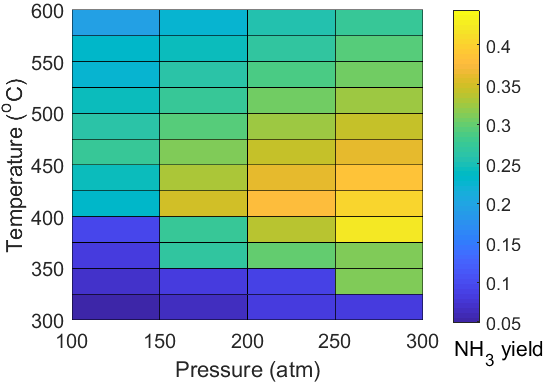
\includegraphics[width=0.3\textwidth]{TPopNEW1}	
			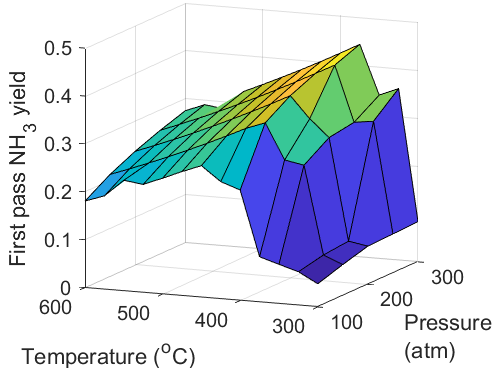
\includegraphics[width=0.3\textwidth]{TPopNEW2}	
			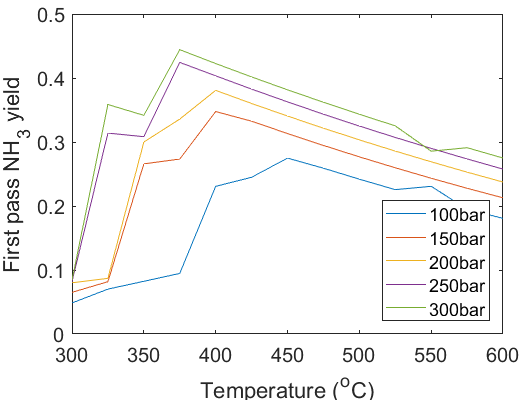
\includegraphics[width=0.3\textwidth]{TPopNEW3}
			\caption{Ammonia single pass yield as function of temperature and pressure}	
		%}
\end{figure}}

\subsubsection{MATLAB Modelling}
MATLAB was used to initialise the model and plot the changes of reactor conditions. This was used to visualise relationships between a small number of variables over a variety of conditions.
\subsubsection{ASPEN simulation}
In order to optimise the pressure and temperature conditions, a number of simulation conditions were trialled using ASPEN plus. Thus measuring the first pass ammonia yield of the reactor at varying operating conditions. Plotting these results shows a peak in NH$_3$ yield at a temperature of 400\textdegree C. Increasing pressure clearly is shown to increase yield, however, above a pressure of 150 bar there is a fall in the rate of increase. From this analysis the reactor operating point was set at $\pbar$bar and $\tc$\textdegree C. This was due to the desire to maximise first pass NH$_3$ yield whilst keeping the plant as economically viable as possible. The flow model used for simulation can be seen in Figure \ref{fig:aspenF}.



%\begin{figure}%
%    \centering
%    
%    \subfloat[label 1]{{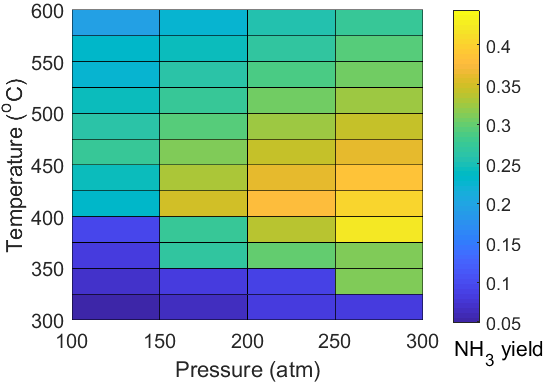
\includegraphics[width=0.2\linewidth]{TPopNEW1} }}%
%    \quad
%    \subfloat[label 2]{{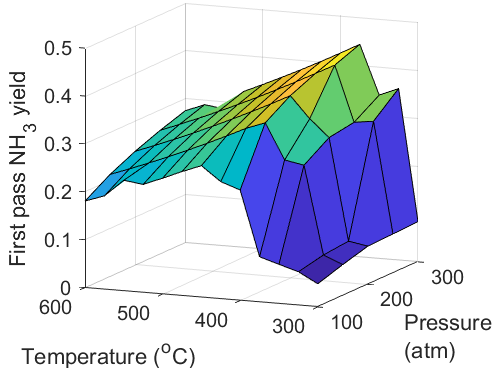
\includegraphics[width=0.2\linewidth]{TPopNEW2} }}%
%    \quad
%    \subfloat[label 2]{{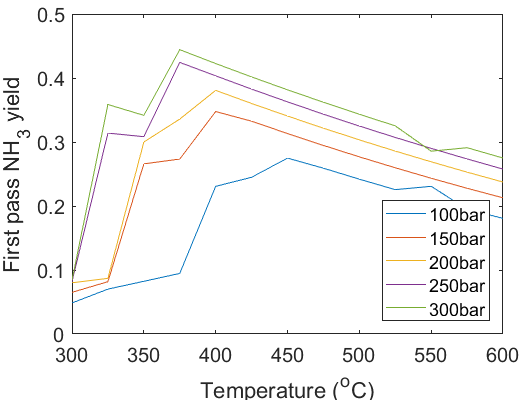
\includegraphics[width=0.2\linewidth]{TPopNEW3} }}%
%    \caption{2 Figures side by side}%
%    \label{fig:example}%
%\end{figure}
%\end{document}

{\centering
	\begin{figure}[!htbp]
		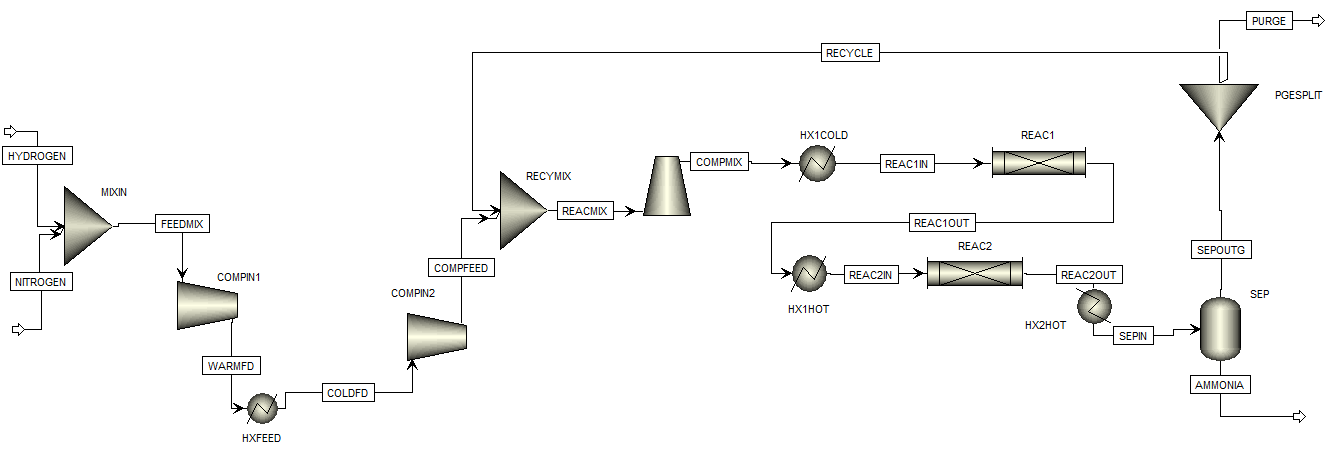
\includegraphics[scale=0.48]{ASPEN_MODEL}
		\caption{ASPEN model of synthesis reaction 	\label{fig:aspenF}}
\end{figure}}
\subsubsection{Model Limitations}
There are a number of limitations of the overall model for the process, the most of important of which are summarised here. 
\begin{itemize}
	\item The lack of a comprehensive process simulation on ASPEN. This is due to the difficulty in matching variable demand data into the simulation. Thus only the synthesis stage was simulated. 
\item The simulation limitations, a number of stages - in particular the ammonia cracker was limited to a rudimentary design. 
\item We have conveniently assumed steady state operation without analysis or process ramping that may be required for maintenance. 
\item The model assumed that yearly average supply was constant and gave no consideration to a growing power demand. 
\end{itemize}
\subsubsection{Plant Control}


The ammonia synthesis process is designed to run at steady state conditions and thus the need for plant control on this process is limited. The overall plant supply/demand matching control has been designed in section \ref{sec:plantscale}. However, to ensure safe operating temperatures of the reactor an emergency quench feed can be used to lower the reactor feed temperature. Above a threshold safe output temperature of T$_{th}$=700\textdegree C a control feed is used to lower the reactant temperature. Energy required for cooling per \textdegree C required is:
\begin{equation}
\frac{\dot{Q}}{T} = \dot{m}C_{p,mix}
\end{equation}

\begin{wrapfigure}{r}{0.22\textwidth}
	%\centering
		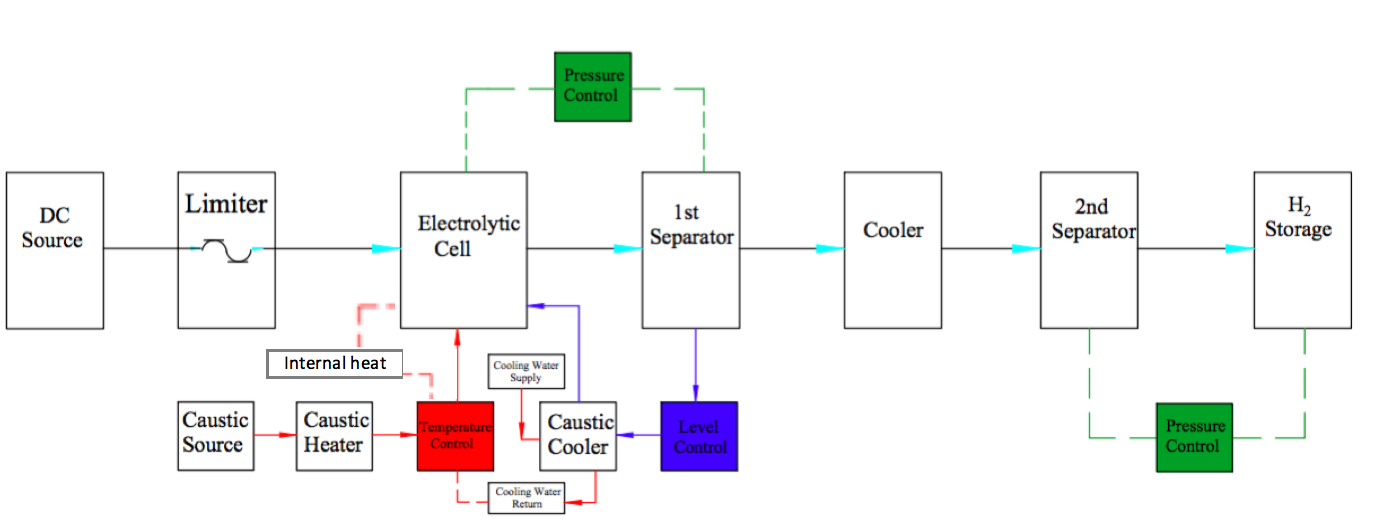
\includegraphics[width=1\textwidth]{control.png}
		\caption{Reactor emergency control \label{fig:controlEMER}}
	%\end{figure}
\end{wrapfigure}
A full control system for the ammonia synthesis process using quench cooling is given by Araujo \cite{Araujo2008}. However, in this design only the emergency reactor control system is considered (Fig. \ref{fig:controlEMER}). 


\subsection{Cost, Sustainability and Safety}

In this section only  the capital cost assessment for the design stage was conducted. For plant operating costs see section \ref{LMCostsection}.
\subsubsection{Capital Cost}
An economic analysis of the ammonia synthesis and storage system requires an assessment of the costs associated with each stage of the design. In this analysis module factor costing method was used for the costing of components \cite{RichardTurtonRichardC.BailieWallaceB.Whiting2013}. Where the purchasing cost $C_p^o$ of equipment in USD is given by the equation \cite{Banares-alcantara2014}:
\begin{equation}
	log_{10}C_p^o = K_1 + K_2log_{10}(A)+K_3(log_{10}(A))^2
\end{equation}
Where $K_1,K_2,K_3$ are defined in Table \ref{tab:Cost}. Thus the bare module cost $C_{BM}$ (direct and indirect costs from purchase and installation) can be calculated from:
\begin{equation}
C_{BM} =C_p^oF_{BM} = C_p^o(B_1+B_2F_MF_P)
\end{equation}
Where $F_M$ and $F_P$ are the respective material and pressure factors and $B_1, B_2$ are constants defined by design. Data for these constraints can be found in data sets and ASME tables \cite{RichardTurtonRichardC.BailieWallaceB.Whiting2013}. The overall capital cost of this stage is estimated to be \$15.5 m with the highest cost being the pre-built ammonia crackers - accounting for over 43\% of process cost.

\begin{table}[!htbp]
	\begin{center}
		
		\caption{Cost summary of all components within the ammonia synthesis and storage process\label{tab:Cost}}
		
		\begin{tabular}{|l|l|l|l|l|l|l|l|}
			\hline
			Component& A & $K_1$   &$K_2$   &$K_3$   & $C_p^o$  & $F_{BM}$ & $C_{BM}$ \\ \hline
			\multicolumn{7}{|c|}{\textbf{Synthesis loop} }& \textbf{\$4.017 m} \\
			\hline
			Reactor                           & 7.16 m$^3$                & 4.0152 & 0.4485     & 0.1074 & \$ 0.005m & 118.18&   \$0.591 m                 \\ \hline 
			Compressors                             & 2541 kW        & 2.2897 & 1.3604         & -0.1027 & \$0.538 m & 5.80 &  \$3.120 m                  \\ \hline 
			Separator                              & 0.636 m$^3$                & 3.4974 & 0.4485         & 0.1074 & \$0.003 m & 118.18 &  \$0.306 m                  \\ \hline 
			\multicolumn{7}{|c|}{\textbf{Storage} } & \textbf{\$4.705 m} \\
			\hline
			Steel Tank                          & 21997 	m$^3$                & 4.8509 & -0.3973         & 0.1445 & \$0.708 m &4.5 &  \$3.186 m              \\ \hline 
			Concrete Tank                          & 26699 m$^3$                & 4.8509 & -0.3973         & 0.1445 & \$0.839 m &1.5 &  \$1.259 m              \\ \hline 
			Compressor                          & 74 kW                & 2.2897 & 1.3604        & -0.1027 & \$0.030 m &4.4 &  \$0.132 m              \\ \hline 
			Condenser                       & 69.2 m$^2$                & 4.0336 & 0.2341         & 0.0497 & \$0.043 m &2.99 &  \$0.129 m              \\ \hline 	
			\multicolumn{7}{|c|}{\textbf{Cracker} } & \textbf{\$6.760 m} \\
			\hline
			Cracker                             & -                & - & -        & - & \$6.760 m & -&     \$6.760 m               \\ \hline 
			\textbf{Total}& - & - &  -   & - &-  & - &  \textbf{\$ 15.482 m} \\ \hline
			
		\end{tabular}
	
	\end{center}
\end{table}
 
\subsubsection{Process Sustainability}
Whilst the overall system sustainability is covered later in this report. The ammonia synthesis and storage stage of this project has been one in which no external inputs have been used besides the environmentally produced hydrogen and nitrogen in order to make liquid ammonia. In addition to this recycling the outlet streams has in some cases increased overall output efficiency by a factor of 3, whilst reducing waste streams.


	\begin{figure}[!htbp]
		\begin{center}

		\label{fig:flowsh}
		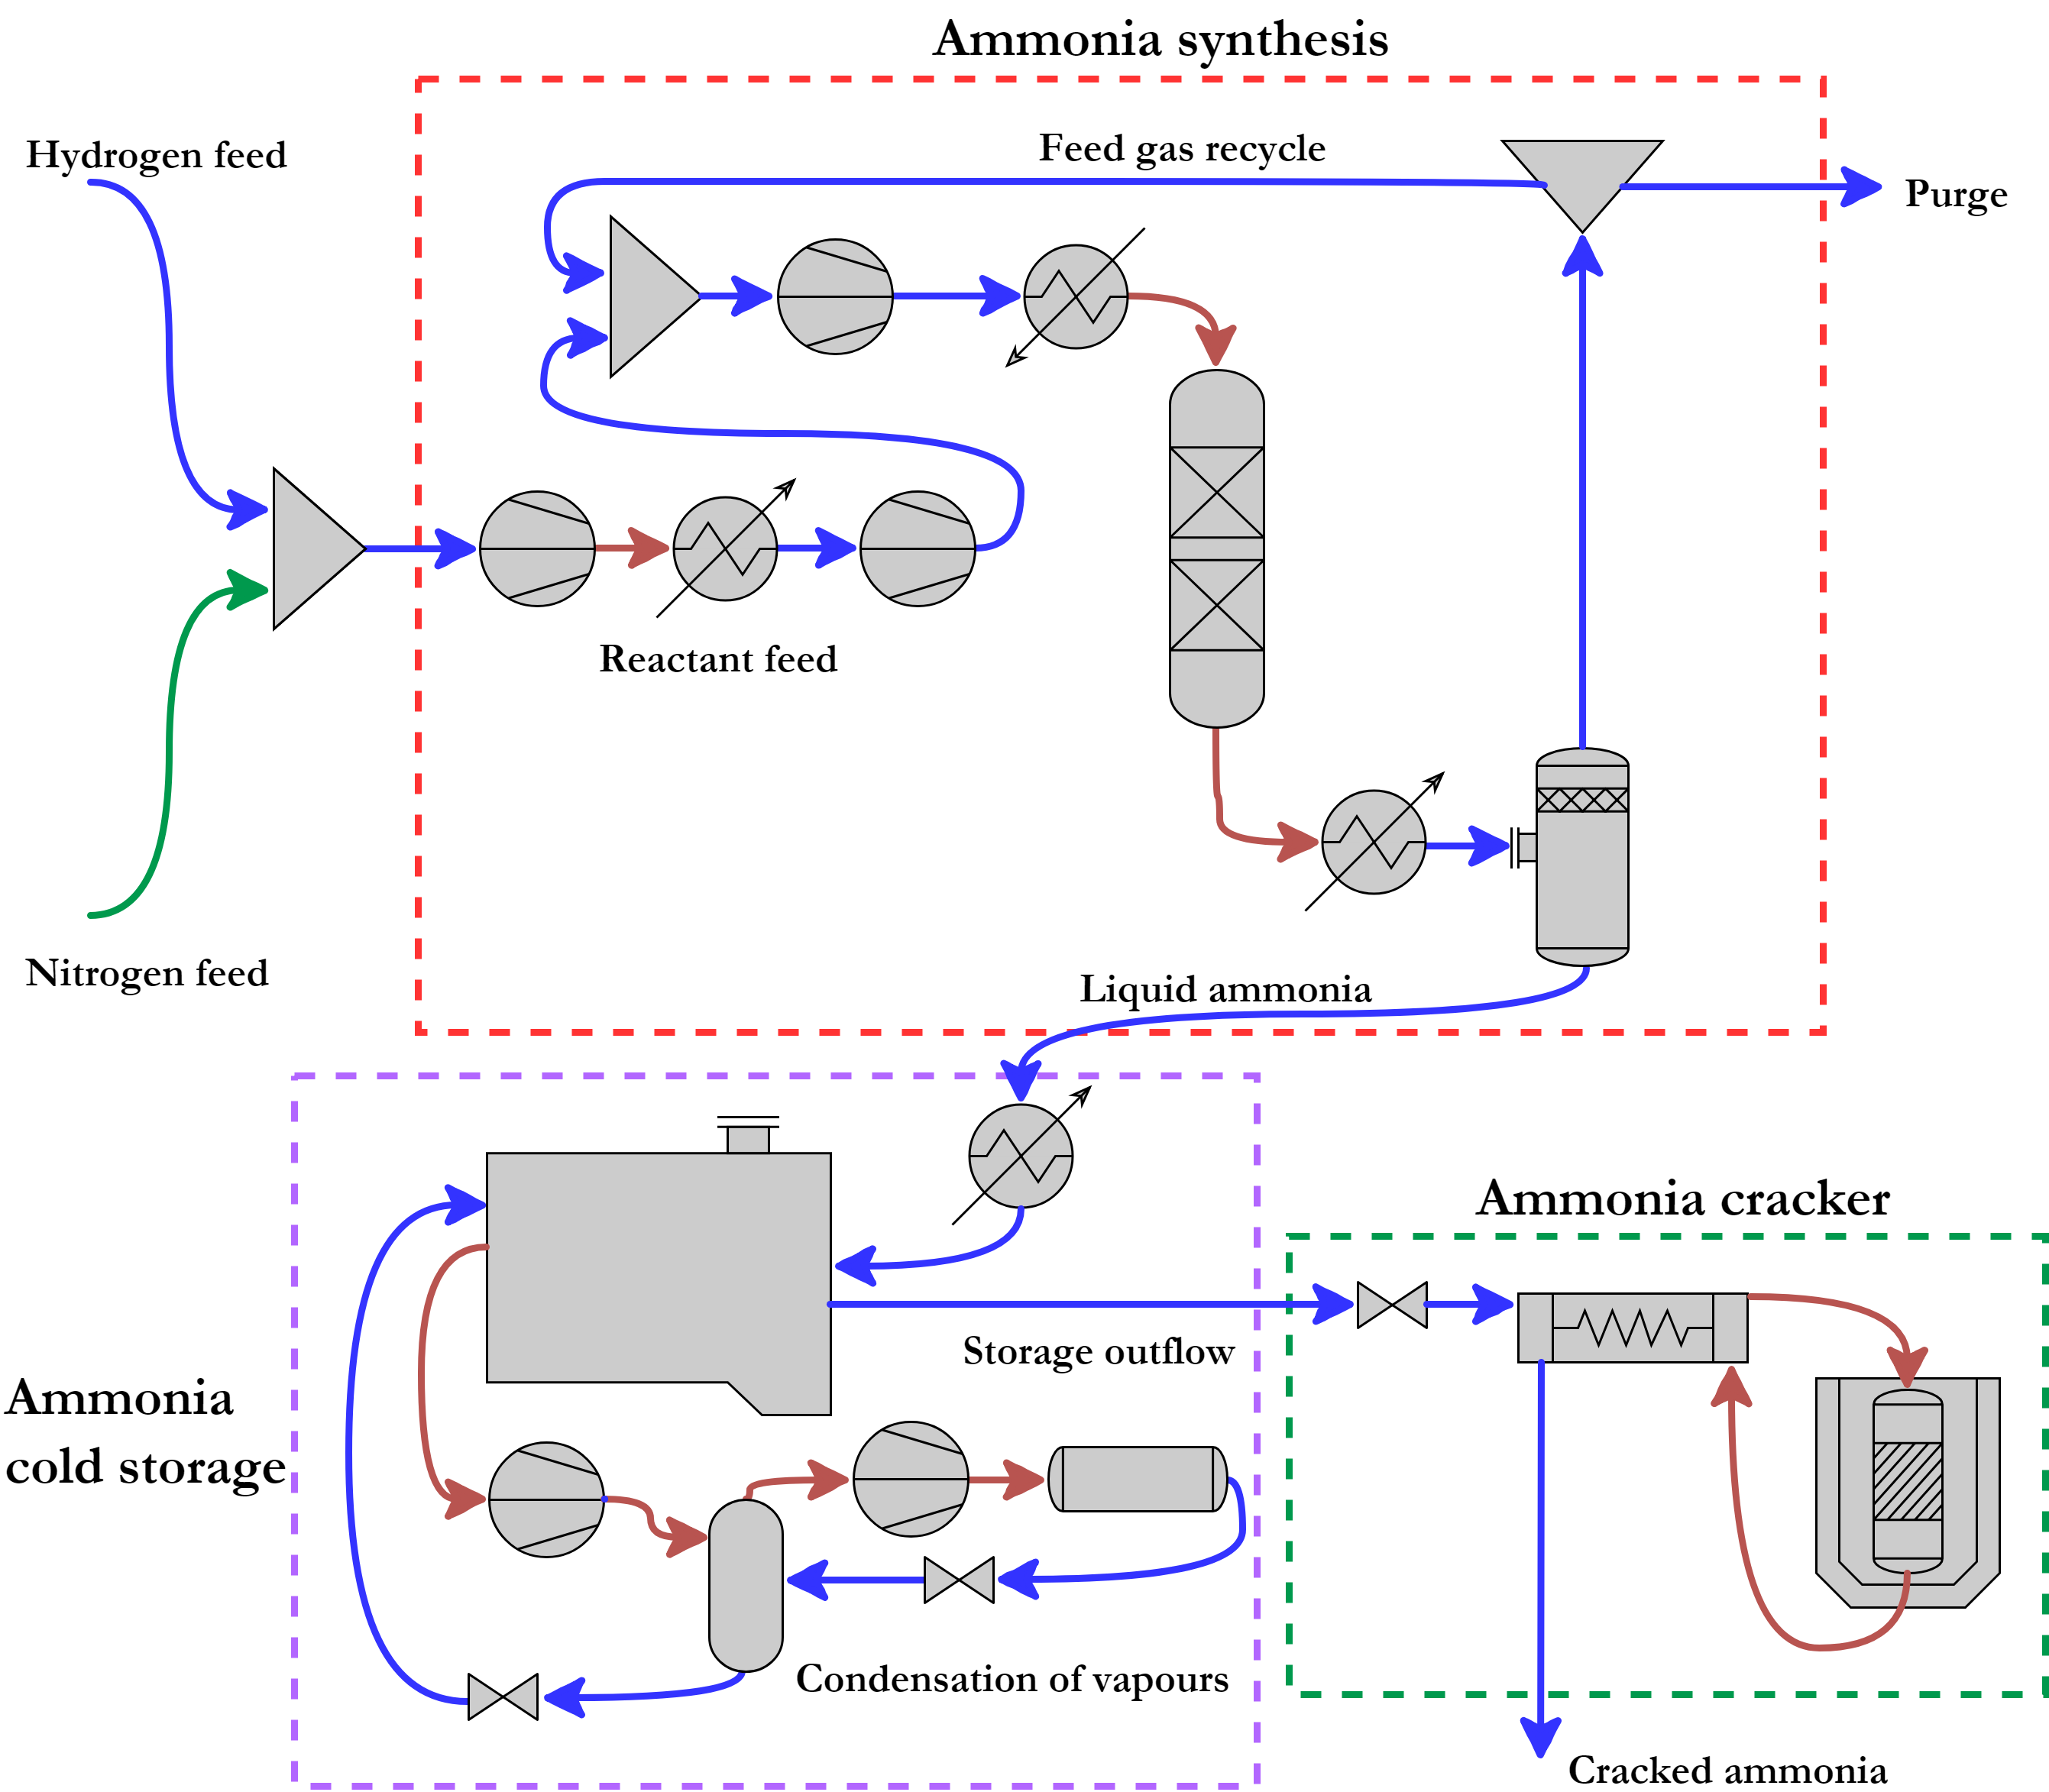
\includegraphics[width=0.85\textwidth]{Flowsheet}
		\caption{Flowsheet of process}
		\end{center}
\end{figure}

\newpage
{\renewcommand{\arraystretch}{0.96}
	\begin{landscape}
		\begin{table}
			\centering
			\caption{HAZOP analysis of synthesis stage}
			\begin{tabular}{|p{1.5cm}|p{1.2cm}|p{5.7cm}|p{5.2cm}|p{8.2cm}|} 
				\hline
				Line           &Dev. & Cause                                                                                                 & Consequences                                                             & Action                                                                                                                             \\ 
				\hline
				Reactor        & No        & Valve stuck/blocked                                                                                   & Rapid temperature change, Catalyst damage, Reaction rate fall.~          & Measure temperature with a thermocouple and flow rate continuously with alarm and shut down system, catalytic testing.~            \\ 
				\hline
				& Less      & \begin{tabular}[c]{@{}l@{}}Low output concentration,\\Reactor leakage,\\Temperature fall\end{tabular} & Release of reactants, fall in output. Explosive ammonia/air mixture.                                     & Measure concentrations of gases outside of the reactor to detect any leakage of reactants. Catalyst replacement.                   \\ 
				\hline
				& More      & \begin{tabular}[c]{@{}l@{}}Overpressure\\Overtemperature\end{tabular}                                 & Vessel failure, release of reactor gases.                           & Pressure and temperature sensors and warnings, complete shutdown at system before critical level reached. Alarm system in place.~  \\ 
				\hline
				H. Exch. & No        & Valve stuck, blockage                                                                                 & Pipe burst - gas leak                                                    & Flow path redundancy in HX.~                                                                                                       \\ 
				\hline
				& Less      & Low heat exchange - damage to surface plate, low flow rate.                                           & Fall in output, damage to HX.                                            & Thermocouple to measure temperature profile of flow. Regular maintenance.                                                          \\ 
				\hline
				& More      & High flow rate, high temperature                                                                      & Overheating of reactor.                                  & Measure flow temperature. Regular maintenance.                                                                                  \\ 
				\hline
				Compr.     & No        & No flow - pump blockage, no power supply, complete pressure loss - leak of compressor                 & Gas leak into atmosphere, reduction in reaction conversion               & Gas monitoring outside chamber, regular maintenance.                                                                               \\ 
				\hline
				& Less      & Low compression level - low power supply/blockage in system                                           & Inefficient operation, damage to pump.                                   & Filter of feed, flow rate and pressure monitoring.                                                                                 \\ 
				\hline
				& More      & Overcompression, power surge, control failure, high flow rate                                         & Damage to compressor pump, pipe rupture. & Power buffer systems. Warning and detection alarms.                                                                                \\ 
				\hline
				Separ.      & No        & No output flow - separator leak                                                                       & No ammonia output, gas leak                                              & Continuous monitoring of pressure, temperature and flow rates. Regular inspection.                                                 \\ 
				\hline
				& Less      & Temperature too high                                                                                  & Mesh damage, low yield.                                       & Regular stream testing. Periodic inspection.                                                                  \\ 
				\hline
				& More      & Temperature too low                                                                                   & Power wastage in cooling.                                        & Thermocouple to measure vessel temperature.                                                                                 \\ 
				\hline
				Storage        & No        & No~                                                                                                   & Failure power generation stages                         & Monitoring of storage levels, low storage warning.                                                                                 \\ 
				\hline
				& Less      & Refrigeration failure of vessel                                                                       & Building up of pressure - burst vessel                                   & Leak before burst design of storage tank. Pressure relief valve.~                                                                  \\ 
				\hline
				& More      & Buildup of pressure in container - failure of gas release valve                                       & Vessel failure/bursting. Explosive ammonia/air mixture.                                                  & Redundancy in~ release valves, regular inspection. Pressure monitoring inside vessel.                                              \\
				\hline
			\end{tabular}
		\end{table}
		
	\end{landscape}
}


\subsection{Section Summary}
\subsubsection{Results and Conclusion}
\begin{wraptable}{r}{0.45\textwidth}
	\singlespacing
	\centering
		\caption{Design summary}
		\begin{tabular}{ |l|l|  }
			
			\hline
			NH$_3$ production rate & 257 tpd\\
			\hline
			NH$_3$ storage capacity & 15000 t \\
			\hline
			Capital cost of process &  \$15.5 m  \\
			\hline
			Single-pass NH$_3$ conversion & 34\% \\
			\hline
			Overall NH$_3$ conversion rate    & 96\% \\
			\hline
			Operating pressure& 150 bar\\
			\hline
			Operating temperature & 400\textdegree C \\
			\hline
			Storage pressure & 1 bar \\
			\hline
			Storage temperature & -33\textdegree C \\
			\hline
		\end{tabular}
\end{wraptable}

During the final design iteration of the synthesis stage a first pass conversion rate of \conv \% can be achieved after optimization. This is achieved at a pressure of \pbar  bar and a reactor inlet temperature of \tc\textdegree C. Figure \ref{fig:aspenF} shows the final stage ammonia synthesis stage ASPEN flow diagram. This is a high first pass conversion relative to industrial averages and is achieved by using high pressure and improved catalyst in relation to the industrial standard. The ammonia synthesis, whilst a well established process requires careful design and optimisation due to the specific design requirements. The use of ASPEN and MATLAB has allowed for the creation of a dynamic modelling system that has enabled the conversion rate of ammonia to be optimised, whilst design of the storage requirements and power generation needs of the plant has enabled this stage to be designed to minimise the waste output of the plant through stream recycles. This achieves an overall conversion rate nearly 3 times than that of a first pass yield. 

In conclusion, this section of the reactor is vital in providing the long term energy storage. This has meant that scale and reliability have been prioritised in the design, whilst minimising environmental impact and maximising economic efficiency. This satisfies the initial design objectives and meets the needs of respective processes elsewhere in the plant. 


\subsubsection{Further Design}
Whilst this design has addressed all the initial requirements, there are further improvements that could be made to the process. One of these would be to design a large scale cracker, this may have led to cost reductions over the current design. Finally, recycling the hydrogen content within the purge stream, would not only reduce output wastage but also improve the overall process efficiency.

\bibliography{./ammoniasynthJR/ammoniasynth/v3bib}
\bibliographystyle{unsrt}
%\end{document}